\documentclass[twoside]{article}
\input{ISC18-english.sty}
\usepackage{graphicx}
\usepackage{subcaption}
\usepackage{caption}
\begin{document}
\thispagestyle{empty}
\fancyhead[LE]{EM Algorithm for Multi-Response Bridge Regression}
\fancyhead[RO]{Masoudi and Ghatari}



\begin{center}
{
\includegraphics [height=25mm, width=150.3mm] {Images/isc18E}} \\
\vspace*{-1.8cm}
% {
\includegraphics [height=25mm, width=150.3mm] {Images/isc18E}} \\
\vspace*{4cm}
{\Large \bf Expectation-Maximization Algorithm for Efficient Optimization of Multi-Response Bridge Regression}\\
\vspace{0.5cm}
{\bf Rozhina Masoudi$^1$, Amir Hossein Ghatari\footnote[1]{{\bf Corresponding Author:} {\tt a.h.ghatari@aut.ac.ir }} \\
	$^1$Department of Statistics, Faculty of Mathematics and Computer Science, Amirkabir University of Technology, Tehran, Iran. 
}
\end{center}
\rule{\textwidth}{0.2mm}



\noindent{\bf Abstract:}\\
Optimizing multi-response bridge regression using conventional methods like Newton-Raphson is computationally expensive and sensitive to initialization. This paper proposes a novel Expectation-Maximization (EM) algorithm for optimizing the multi-response bridge objective. By interpreting the Generalized Gaussian prior as a Gaussian Scale Mixture, we derive an iterative reweighted least squares procedure with a straightforward M-step. Numerical experiments show that EM outperforms Newton-Raphson in most cases. The two methods give similar sparsity patterns. However, EM achieves lower prediction error on average. 



\noindent{\bf Keywords:} 
EM algorithm, Multi-response, Penalized regression, Feature selection. \\
\noindent{\bf Mathematics Subject Classification (2010):} $\rm 62J05$, $\rm 62J12$ \\
\rule{\textwidth}{0.2mm}



\section{Introduction}
Penalized regression in high-dimensional settings (more predictors than observations) aims to jointly select features and estimate coefficients. A common but suboptimal approach for multi-response problems fits separate univariate models for each response \cite{breiman1997}. This ignores correlations among responses, discarding valuable data structure and causing loss of statistical efficiency and suboptimal feature selection. A proper multi-response framework must explicitly account for these dependencies to fully leverage joint information from all responses.



\cite{ghatari2024} proposed the multi-response bridge regression to overcome this limitation. Their model uses a Mahalanobis norm with covariance \(\Sigma\) to handle response correlations. They also introduced MGIC criteria for parameter selection and proved identifiability. However, their optimization relied on conventional methods like Newton-Raphson (similar to \cite{fan2001}). These approaches face convergence speed, numerical stability, and scalability issues, particularly for non-convex penalties (\(\alpha < 1\)).
Optimizing penalized likelihood functions has been a central challenge in statistics. \cite{fan2001} proposed Local Quadratic Approximation (LQA) for non-concave penalties. \cite{efron2004} introduced Least Angle Regression (LARS) for LASSO. Coordinate descent methods are also popular \cite{tibshirani1996}. Recently, \cite{kittisuwan2022} studied minimax-concave penalties for double thresholds, and \cite{kittisuwan2023} investigated fused lasso for signal enhancement.



 In this paper, we propose an alternative optimization strategy using Expectation-Maximization (EM) algorithm. By formulating the bridge penalty as a Gaussian Scale Mixture (GSM), we derive an iterative reweighted least squares procedure that is both intuitive and numerically stable. This approach provides a unified and efficient framework for optimizing the multi-bridge objective, demonstrably improving upon the computational aspects of earlier implementations.



\section{Theoretical Foundations}



\subsection{Multivariate Linear Regression Model}
Consider the standard multivariate linear regression model where we have \(n\) observations, \(p\) predictors, and \(K\) response features. Let \(Y \in \mathbb{R}^{n \times K}\) be the matrix of responses, \(X \in \mathbb{R}^{n \times p}\) be the design matrix, and \(E \in \mathbb{R}^{n \times K}\) be the matrix of random errors. The model is expressed as:
\begin{equation}\label{eq:obj1}
Y = X B + E,
\end{equation}
where \(B \in \mathbb{R}^{p \times K}\) is the coefficient matrix. A fundamental assumption in multivariate analysis is that the rows of the error matrix, \(E^{(i)} \in \mathbb{R}^K\), are independently and identically distributed according to a multivariate normal distribution with zero mean and a \(K \times K\) covariance matrix \(\Sigma\), i.e., \(E^{(i)} \sim \mathcal{N}_K(\mathbf{0}, \Sigma)\). Ignoring the structure of \(\Sigma\) (e.g., by fitting separate models for each column of \(Y\)) is equivalent to assuming \(\Sigma\) is diagonal, which leads to a loss of information when the response variables are correlated \cite{ghatari2024}.



\subsection{Multi-Response Bridge (Multi-Bridge) Regression}
\cite{ghatari2024} proposed the multi-bridge regression model to simultaneously handle variable selection and inter-response correlation. The objective function is defined as
\begin{equation}\label{eq:obj}
Q^{*}(\lambda ,B_{\lambda}) = \frac{1}{Kn}\sum_{i = 1}^{n}(Y^{(i)} - B_{\lambda}^{T}X_{i})^{T}\Sigma^{-1}(Y^{(i)} - B_{\lambda}^{T}X_{i}) + \lambda \sum_{j=1}^{p}\sum_{k=1}^{K}|\beta_{jk}^{\lambda}|^{\alpha},
\end{equation}
where ($ 0 \leq \alpha \leq 2 $). This formulation includes the multi-LASSO (($ \alpha $=1)) and multi-Ridge (($ \alpha $=2)) as special cases. The penalty term encourages sparsity in ($B_ \lambda $), while ($ \Sigma^{-1} $) accounts for the correlation structure among responses.



\subsection{Information Criteria for Regularization Parameter Selection}



Selecting the regularization parameter ($ \lambda $) is crucial for model performance. Extending the generalized information criterion framework of \cite{zhang2010} to the multivariate setting, \cite{ghatari2024} proposed the MGIC. Two important members of this family are the Multivariate BIC (MBIC)
\[
\text{MBIC}(\lambda) = \log(\det(S_{e_\lambda})) + \frac{\sqrt[3]{n} \cdot df_\lambda}{Kn},
\]
and the Multivariate AIC (MAIC)
\[
\text{MAIC}(\lambda) = \log\left(\frac{1}{n}\sum_{i=1}^n e_i^T S_{e_\lambda}^{-1} e_i\right) + \frac{2 G_2(Y, \hat{B}_\lambda) df_\lambda}{Kn},
\]
where $S_{e_\lambda} = \frac{1}{n} e_\lambda^T e_\lambda$, $e_\lambda = Y - X\hat{B}_\lambda$, and $df_\lambda = \#\{j,k: \hat{\beta}_{jk}^\lambda \neq 0\}$. These criteria provide a data-driven approach for selecting the optimal $ \lambda $ by balancing model fit and complexity.



\subsection{Definition of the EM Algorithm}
The Expectation-Maximization (EM) algorithm is an iterative method for obtaining maximum likelihood or maximum a posteriori (MAP) estimates in latent variable models. Each iteration consists of two steps:
\begin{enumerate}
	\item \textbf{E-step (Expectation):} Compute the expected complete-data log-posterior with respect to the conditional distribution of the latent variables given the observed data and current parameter estimates.
	\item \textbf{M-step (Maximization):} Maximize the resulting expected complete-data log-posterior (\(Q\)-function) to update the parameter estimates.
\end{enumerate}
For penalized regression models, the EM algorithm can be formulated by interpreting the penalty term as a prior distribution on the coefficients. This leads to a sequence of simpler optimization problems, often in the form of weighted least squares.



\section{EM Algorithm for Multi-Response Bridge Regression}
From a Bayesian perspective, minimizing \(Q^*\) in (\ref{eq:obj}) is equivalent to a Maximum A Posteriori estimate. Following \cite{lindley1971}, the regularized objective corresponds to a posterior distribution. \cite{ghatari2024} showed that the negative log-likelihood of model (\ref{eq:obj1}) is:
\[
-\log L(Y|X,B_\lambda) \propto \frac{1}{Kn}\sum_{i=1}^n (Y^{(i)} - B_\lambda^T X_i)^T \Sigma^{-1} (Y^{(i)} - B_\lambda^T X_i),
\]
and the penalty corresponds to a negative log-prior. We place an independent Generalized Gaussian prior on each coefficient. 
Thus, the posterior satisfies \( \log p(B_\lambda \mid Y,X) \propto -Q^*(B_\lambda)\).
\subsection*{E-Step (Expectation)}
Define the \(Q\)-function:
$$ Q(B_\lambda | B_\lambda^{(t)}) = \mathbb{E}_{\tau^2 | Y, B_\lambda^{(t)}} \left[ \log P(B_\lambda, \tau^2 | Y) \right] $$
Using properties of the generalized inverse Gaussian distribution:
$$ w_{jk}^{(t)} := \mathbb{E}\left[ \frac{1}{\tau_{jk}^2} \Big| Y, B_\lambda^{(t)} \right] = \alpha \lambda |\beta_{jk}^{\lambda, (t)}|^{\alpha-2} $$
Thus:
$$ Q(B_\lambda | B_\lambda^{(t)}) = -f(B_\lambda) - \frac{1}{2} \sum_{j=1}^p \sum_{k=1}^K w_{jk}^{(t)} (\beta_{jk}^\lambda)^2 + \text{const} $$



\subsection*{M-Step (Maximization)}
We maximize \(Q(B_\lambda | B_\lambda^{(t)})\) with respect to \(B_\lambda\). Taking the derivative and setting to zero:
$$ -\nabla f(B_\lambda) - W^{(t)} \odot B_\lambda = 0 $$
where \(\odot\) denotes the Hadamard product, and \(W^{(t)}\) has elements \(w_{jk}^{(t)}\).



Substituting \(\nabla f(B_\lambda) = -\frac{2}{Kn} X^T (Y - X B_\lambda) \Sigma^{-1}\):
$$ \frac{2}{Kn} X^T X B_\lambda \Sigma^{-1} + W^{(t)} \odot B_\lambda = \frac{2}{Kn} X^T Y \Sigma^{-1} $$



\subsection{Update Equation and Algorithm}
The fixed-point iteration for the EM algorithm is:
$$ \frac{2}{Kn} X^T X B_\lambda^{(t+1)} \Sigma^{-1} + W^{(t)} \odot B_\lambda^{(t+1)} = \frac{2}{Kn} X^T Y \Sigma^{-1} $$
where \(w_{jk}^{(t)} = \alpha \lambda |\beta_{jk}^{\lambda, (t)}|^{\alpha-2}\). Therefore, \(\beta_{jk}^{\lambda, (t)} = \left( \frac{w_{jk}^{(t)}}{\alpha \lambda} \right)^{\frac{1}{\alpha-2}}\).
The final EM algorithm \ref{alg1} for the problem becomes: \pagebreak
{ \linespread{0.5} \hrule
\begin{alg}\label{alg1}
EM Algorithm for Multi-Response $L_\alpha$-Regularized Regression:
\begin{itemize}
\item \textbf{Input:} $X \in \mathbb{R}^{n \times p}$, $Y \in \mathbb{R}^{n \times K}$, $\Sigma \in \mathbb{R}^{K \times K}$, $\alpha \in (0,2]$, $\lambda > 0$, tolerance $\epsilon > 0$, max iterations $T_{\max}$, stability $\delta = 10^{-8}$
\item \textbf{Output:} $\hat{B}_\lambda \in \mathbb{R}^{p \times K}$ (optimal coefficient matrix)
\item Initialize $t = 0$, $B_\lambda^{(0)} = \mathbf{0}_{p \times K}$
\item Precompute $A = \frac{2}{Kn} X^T X$ and $C = \frac{2}{Kn} X^T Y \Sigma^{-1}$
\item While $t < T_{\max}$:
\begin{itemize}
\item \textbf{E-step:} For $j = 1$ to $p$ and $k = 1$ to $K$:
$$ b = \max(|\beta_{jk}^{(t)}|, \delta), \quad w_{jk}^{(t)} = \alpha \lambda \cdot b^{\alpha-2} $$
\item \textbf{M-step:} Solve $A B_\lambda^{(t+1)} \Sigma^{-1} + W^{(t)} \odot B_\lambda^{(t+1)} = C$ for $B_\lambda^{(t+1)}$
\item \textbf{Convergence check:} If $\|B_\lambda^{(t+1)} - B_\lambda^{(t)}\|_F < \epsilon \|B_\lambda^{(t)}\|_F$, break
\item $t = t + 1$
\end{itemize}
\item Return $\hat{B}_\lambda = B_\lambda^{(t)}$
\end{itemize}
\end{alg} \hrule}



\subsection{Special Cases: EM for Lasso Version}
For \(\alpha = 1\), the general EM algorithm reduces to the Adaptive Lasso formulation.



\textbf{E-step:} The weights are updated according to
$$
w_{jk}^{(t)}
=
\frac{\lambda}
{\max\!\left(|\beta_{jk}^{(t)}|,\epsilon\right)},
\qquad
\epsilon = 10^{-6}.
$$



\textbf{M-step:} The coefficient matrix is obtained by solving
$$
\frac{2}{Kn}X^TX B_\lambda^{(t+1)}\Sigma^{-1}
+
W^{(t)} \odot B_\lambda^{(t+1)}
=
\frac{2}{Kn}X^TY\Sigma^{-1},
$$
where \(W^{(t)}=(w_{jk}^{(t)})\).  \\



{ \linespread{0.5} \hrule
	\begin{alg}\label{alg2}
\textbf{EM Algorithm for Lasso (\(\alpha = 1\)):}
\begin{itemize}
	\item Initialize \(B_\lambda^{(0)} = \mathbf{0}_{p \times K}\)
	\item Repeat until convergence:
	\begin{itemize}
		\item \textbf{E-step:} Compute \(w_{jk}^{(t)} = \lambda / \max(|\beta_{jk}^{(t)}|, \epsilon)\)
		\item \textbf{M-step:} Solve \(A B_\lambda^{(t+1)} \Sigma^{-1} + W^{(t)} \odot B_\lambda^{(t+1)} = C\) with \(A = \frac{2}{Kn} X^T X\) and \(C = \frac{2}{Kn} X^T Y \Sigma^{-1}\)
	\end{itemize}
	\item Return \(B_\lambda^{(t+1)}\)
\end{itemize} \end{alg} \hrule}
\vspace{0.2cm}
Compared with Newton-Raphson, the proposed EM algorithm avoids Hessian calculations and is better suited for non-convex penalties. Since the resulting estimate ($ \hat{B}_{\lambda} $) affects information criteria, different optimization methods may lead to different regularization parameter selections. These effects are examined in the numerical studies.





\section{Numerical Study}



Following the structure of \cite{ghatari2024}, we generate data from the bivariate response model $Y = XB + E$ with $K=2$. The design matrix $X$ is drawn from a multivariate normal distribution with Toeplitz covariance $\Gamma_{ij} = \rho_X^{|i-j|}$, where $\rho_X$ takes values $0.25$, $0.50$, and $0.75$ to control the correlation among predictors. The coefficient matrix $B = [B_1|B_2]$ is set such that $B_1$ has five nonzero entries equal to $3$ and $B_2$ has ten nonzero entries equal to $4$, leaving the remaining coefficients zero, resulting in a total of $10$ relevant features. The error matrix $E$ follows a bivariate normal distribution with mean zero and covariance $\Sigma = \begin{pmatrix}1&0.5\\0.5&1\end{pmatrix}$, inducing correlation between the two responses. We consider sample sizes $n = 200$ and $400$, and predictor dimensions $p = 40$ and $120$. Each simulation setting is replicated $500$ times for training, with an additional test set of size $100$ for evaluation. Note that we consider $\alpha=1$ in  $Q^*(\lambda, B_\lambda)$ and then we have Lasso type of multi-bridge model for simulation which called multi-Lasso.



For each dataset, we optimize $Q^*(\lambda, B_\lambda)$ over a $\lambda$-grid using both NR and EM, and select the optimal $\lambda$ using MAIC, MBIC, 5-fold CV, BIC, and GCV (see \citealp{variyath2020}). We compare EM and NR based on two criteria: (i) the number of selected variables (sparsity), and (ii) the test $\mathrm{MSE_{MH}}$, which measures prediction accuracy while accounting for response correlations. Models are evaluated on the test set using:
\[
\mathrm{MSE_{MH}} = \frac{1}{n_{\text{test}}} \sum_{i=1}^{n_{\text{test}}} e_i^T S_{e_\lambda}^{-1} e_i.
\]
The boxplots in Figure~\ref{fig:comparison} compare the sparsity patterns of EM and Newton-Raphson (NR). Both algorithms maintain sparsity, but occasionally violate the Occam's razor principle by either omitting some true relevant variables or including irrelevant ones. For EM, the number of selected variables decreases as $\rho_X$ increases, with lower variability for $p=40$ and higher variability for $p=120$. GCV and CV select more variables than BIC and MBIC across all settings. For NR, a similar pattern is observed, but NR selects slightly more variables than EM when $\rho_X = 0.25$ and $p = 120$, indicating greater sensitivity to correlation. Increasing $n$ from $200$ to $400$ reduces variability for both methods, improving stability.
\begin{figure}[htbp]
	\centering
	\begin{subfigure}[b]{0.49\textwidth}
		\centering
		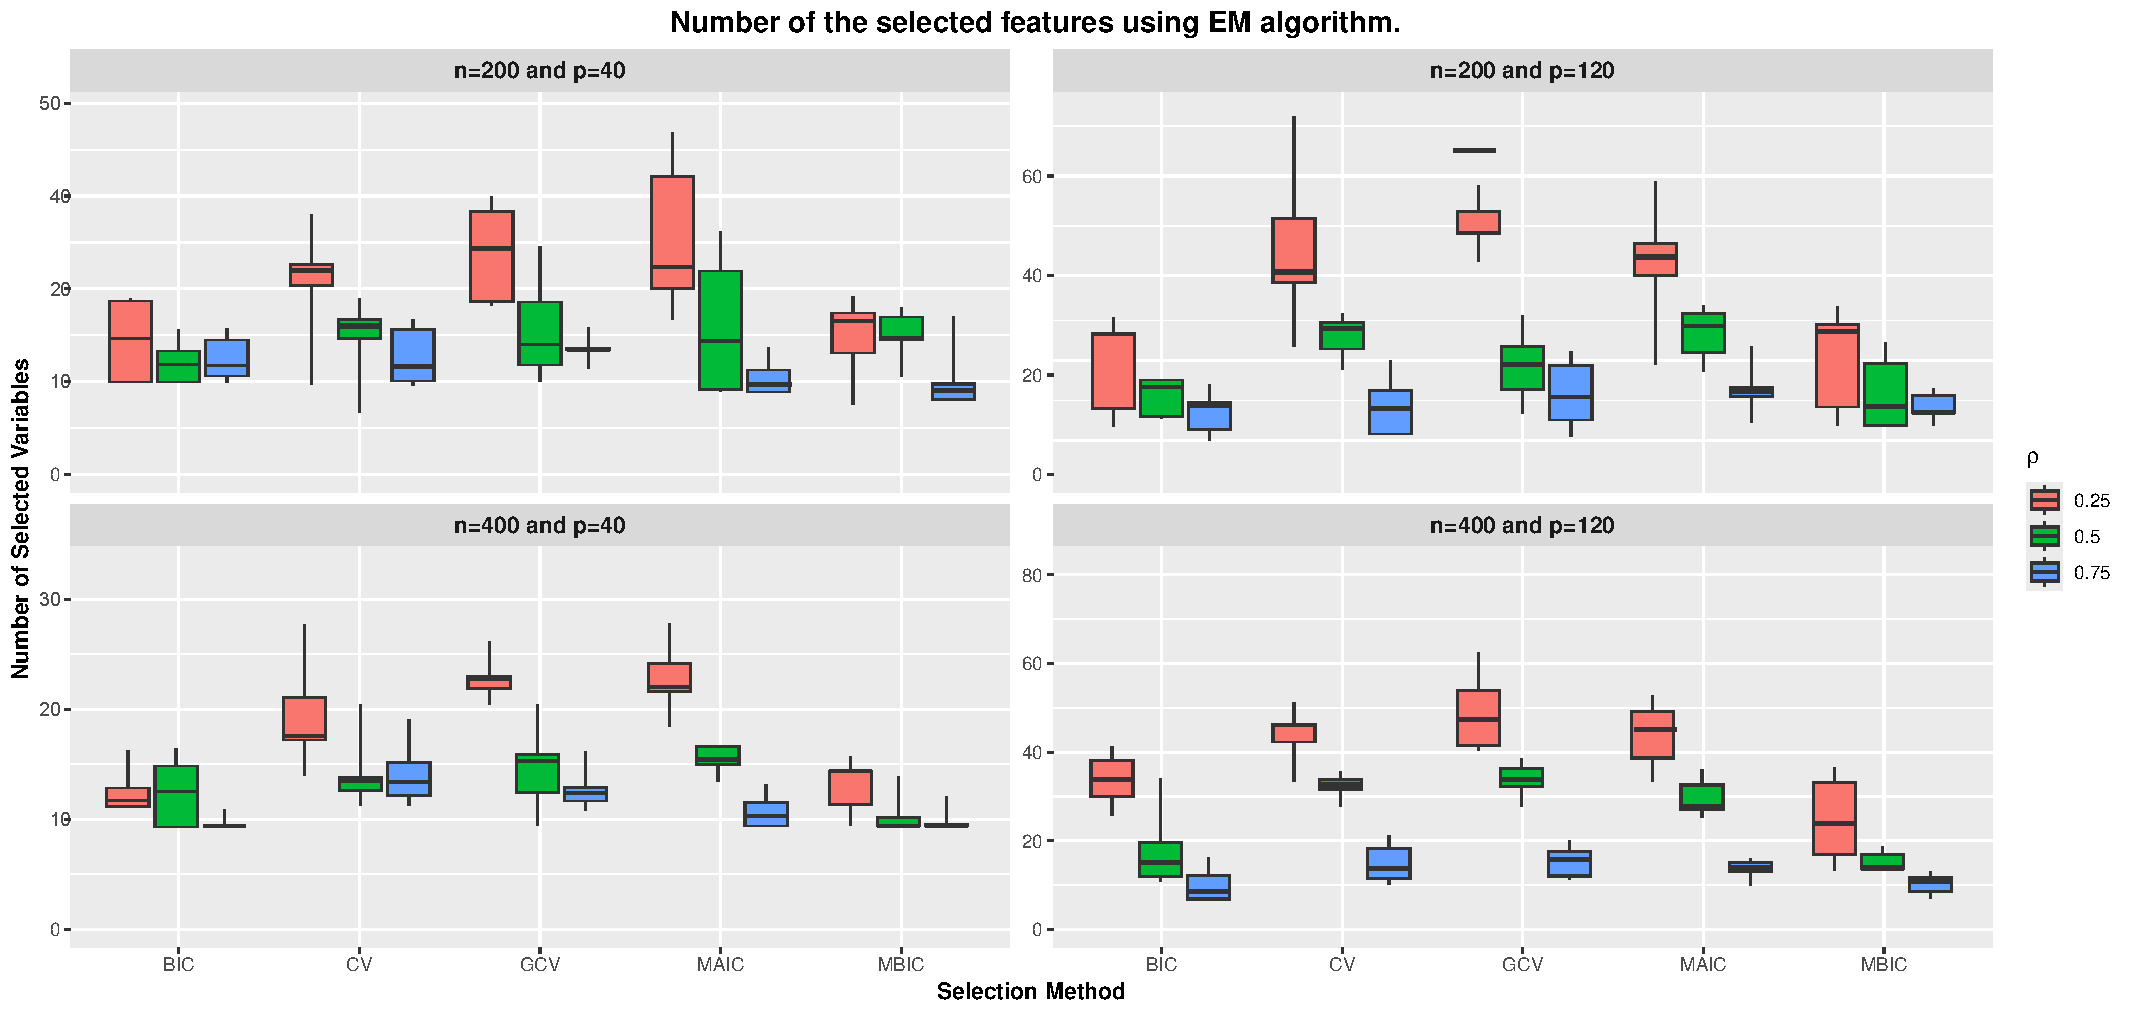
\includegraphics[width=\textwidth]{box-EM.pdf}
		\label{fig:em}
	\end{subfigure}
	\hfill
	\begin{subfigure}[b]{0.49\textwidth}
		\centering
		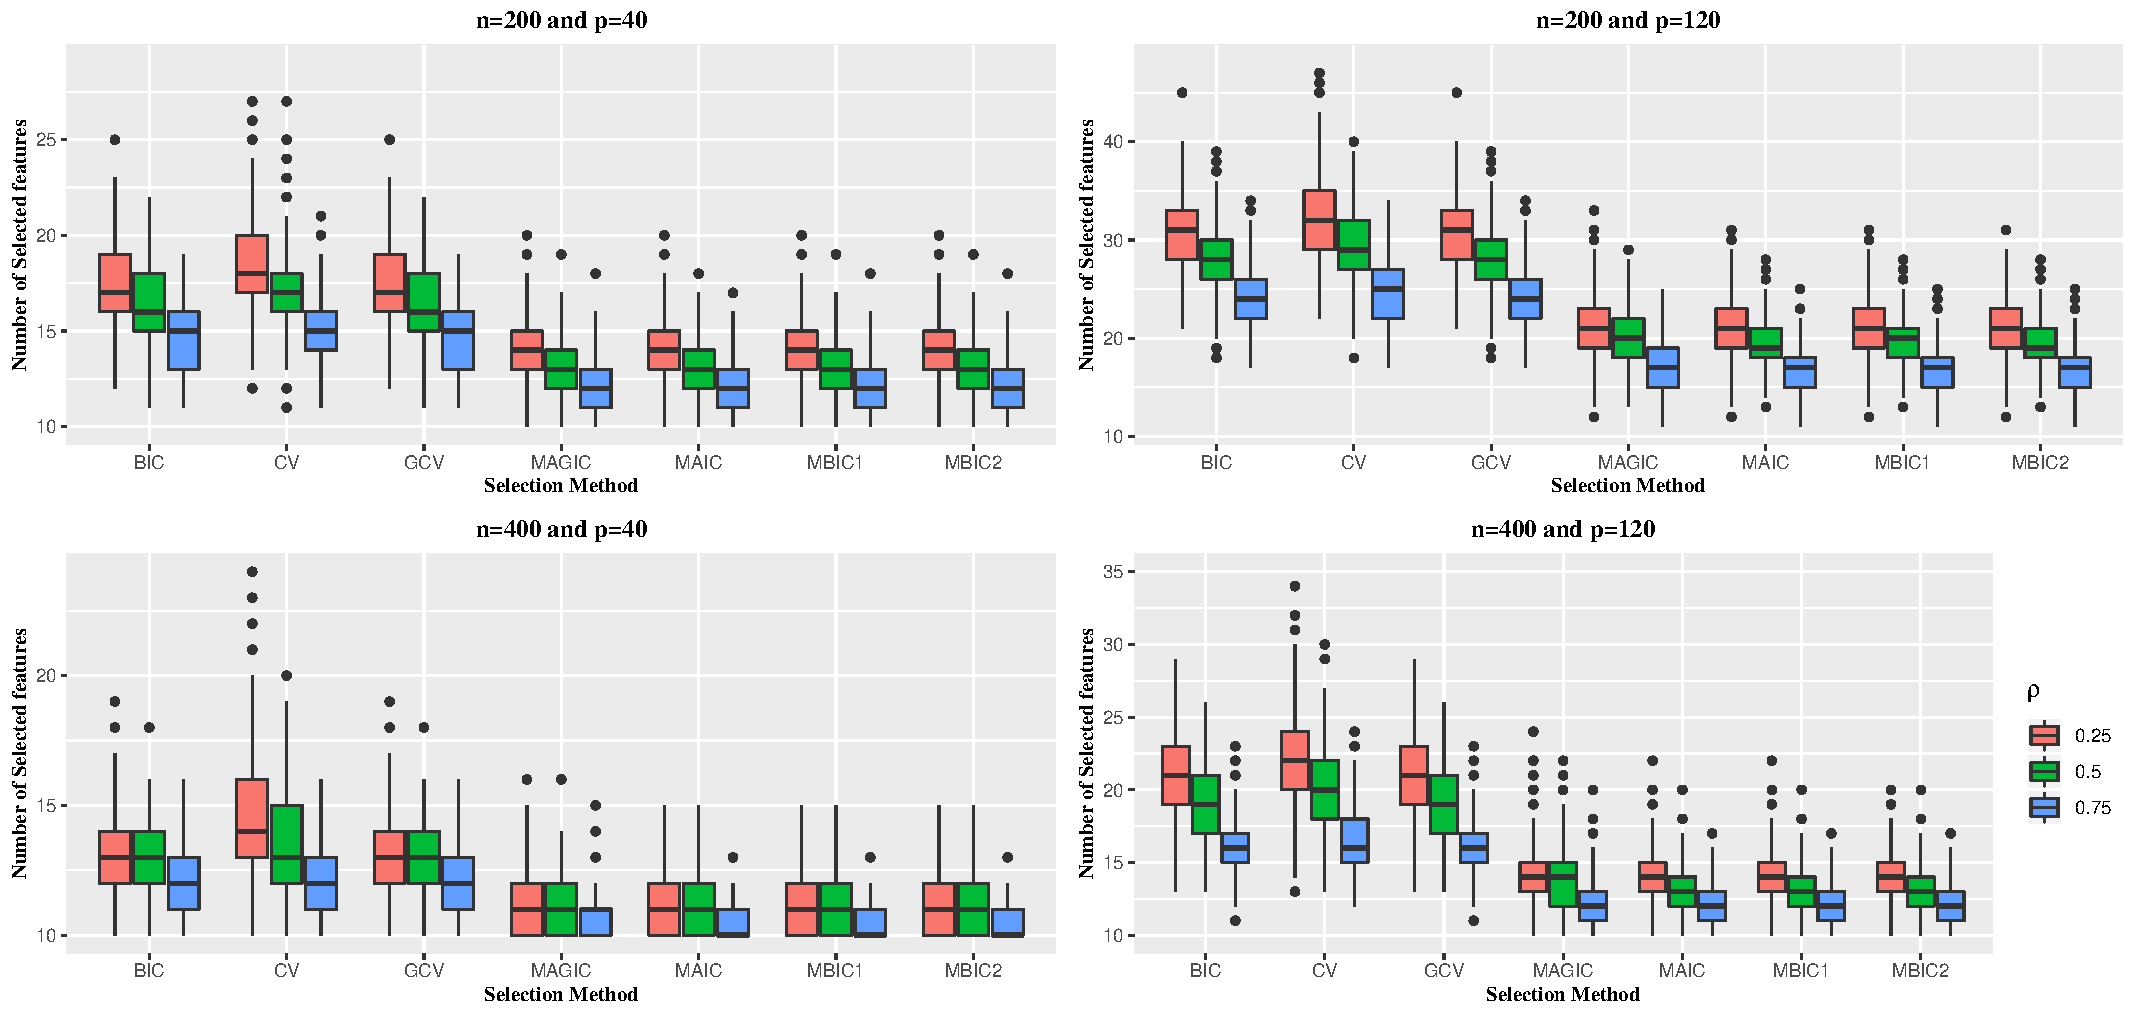
\includegraphics[width=\textwidth]{box1.pdf}
		\label{fig:nr}
	\end{subfigure}
	\caption{Comparison of EM (a) and Newton-Raphson (b) for variable selection.}
	\label{fig:comparison}
\end{figure}



Table~\ref{tab:lasso_comparison} compares the mean test $\mathrm{MSE_{MH}}$ for EM and Newton-Raphson (NR) under the Lasso case ($\alpha=1$). When $n=400$ and $p=40$, both algorithms perform similarly. However, EM improves CV performance across most of the scenarios, reducing $\mathrm{MSE_{MH}}$ as much as $0.03$ (e.g., $1.28$ vs $1.31$ at $\rho_X=0.25$, $n=200$, $p=120$). For BIC and GCV, differences are negligible, as these criteria directly depend on the multi-bridge objective function. Totally, EM shows better performance in high-dimensional settings ($p=120$) with low to moderate correlation.
\begin{table}[h!]
	\centering
	\small
\caption{Mean $\mathrm{MSE_{MH_{test}}}$ values for selected models in the multi-Lasso over 500 iterations.}
	\label{tab:lasso_comparison}
	\begin{tabular}{ccc|ccccc|ccccc}
	%	\hline
		\multicolumn{3}{c}{} & \multicolumn{5}{c}{\textbf{Newton-Raphson}} & \multicolumn{5}{c}{\textbf{EM}} \\
		\cline{1-13}
		\multicolumn{1}{c}{$\rho_X$} & \multicolumn{1}{c}{$n$} & \multicolumn{1}{c|}{$p$} & MAIC & MBIC & GCV & BIC & CV & MAIC & MBIC & GCV & BIC & CV \\
		\hline %\hline
0.25 & 200 & 40  & 1.12 & 1.12 & 1.15 & 1.15 & 1.16 & 1.10  & 1.10  & 1.15  & 1.14  &  1.15 \\
	 &  & 120 & 1.18 & 1.19 & 1.29 & 1.30 & 1.31 &  1.17 & 1.20  & 1.29  &  1.29 & 1.28  \\ \cline{2-13}
	 & 400 & 40  & 1.09 & 1.10 & 1.11 & 1.11 & 1.12 &  1.05 & 1.05  &  1.13 &1.13   &  1.09 \\ 	
	 &  & 120 & 1.13 & 1.12 & 1.18 & 1.18 & 1.20 & 1.11  &  1.11 & 1.19  &  1.19 & 1.17  \\
		\hline
		0.50 & 200 & 40  & 1.11 & 1.11 & 1.14 & 1.14 & 1.14 & 1.11  & 1.10  & 1.13  &  1.13 & 1.11  \\
 &  & 120 & 1.17 & 1.17 & 1.26 & 1.27 & 1.28 & 1.17  & 1.17  &  1.29 & 1.29  & 1.25  \\ \cline{2-13}
 & 400 & 40  & 1.09 & 1.09 & 1.10 & 1.11 & 1.11 & 1.06  & 1.06  & 1.11  &  1.11 &  1.10 \\
 &  & 120 & 1.11 & 1.12 & 1.17 & 1.17 & 1.18 & 1.10  & 1.10  &  1.17 &1.18 & 1.15  \\
		\hline
		0.75 & 200 & 40  & 1.10 & 1.10 & 1.13 & 1.12 & 1.13 & 1.09  & 1.10  &  1.13 & 1.13  & 1.12  \\
 &  & 120 & 1.15 & 1.15 & 1.23 & 1.22 & 1.23 &  1.11 & 1.11  &  1.22 & 1.22  & 1.12  \\\cline{2-13}
 & 400 & 40  & 1.08 & 1.09 & 1.10 & 1.10 & 1.10 & 1.07  & 1.07  &  1.11 & 1.11  &  1.09 \\
 & & 120 & 1.10 & 1.10 & 1.14 & 1.15 & 1.15 & 1.10  &  1.11 &  1.15 &   1.15& 1.12  \\
		\hline
	\end{tabular}
\end{table}



In summary, EM and Newton-Raphson perform similarly in low-dimensional settings. However, EM tends to perform better in high-dimensional scenarios ($p=120$) with low to moderate correlation, especially in CV prediction accuracy. EM also shows more stable sparsity patterns and lower sensitivity to correlation. These features make EM a robust alternative for multi-bridge regression. Furthermore, for MAIC and MBIC, the mean differences between EM and NR are statistically significant based on paired t-tests when n = 400 and p = 40 for each $\rho_X$. 



\section*{Conclusion}
 In this paper, we introduced an Expectation-Maximization algorithm for the multi-response bridge regression model. By formulating the bridge penalty as a Gaussian scale mixture, we obtained an iterative reweighted least squares procedure that is both efficient and stable. Future work includes extending this optimization approach to other penalized regression problems and incorporating more rigorous theoretical results to further improve performance. Due to space limitations, these extensions could not be addressed here.



\begin{thebibliography}{9}



\bibitem[Ghatari and Aminghafari (2024)]{ghatari2024}
Ghatari, A. H. and Aminghafari, M. (2024). Multi-Response Bridge Regularization Parameter Selection via Multivariate Generalized Information Criterion. \emph{Fluctuation and Noise Letters}, 23(4), 2450056.



\bibitem[Breiman and Friedman (1997)]{breiman1997}
Breiman, L. and Friedman, J. H. (1997). Predicting multivariate responses in multiple linear regression. \emph{Journal of the Royal Statistical Society: Series B (Statistical Methodology)}, 59(1), 3-54.



\bibitem[Fan and Li (2001)]{fan2001}
Fan, J. and Li, R. (2001). Variable selection via nonconcave penalized likelihood and its oracle properties. \emph{Journal of the American Statistical Association}, 96(456), 1348-1360.



\bibitem[Efron et al. (2004)]{efron2004}
Efron, B., Hastie, T., Johnstone, I., and Tibshirani, R. (2004). Least angle regression. \emph{The Annals of Statistics}, 32(2), 407-499.



\bibitem[Tibshirani (1996)]{tibshirani1996}
Tibshirani, R. (1996). Regression shrinkage and selection via the lasso. \emph{Journal of the Royal Statistical Society: Series B (Methodological)}, 58(1), 267-288.



\bibitem[Kittisuwan and Thaiwirot (2022)]{kittisuwan2022}
Kittisuwan, P. and Thaiwirot, W. (2022). Novel non-convex regularization for generating double threshold value in penalized least squares regression. \emph{Fluctuation and Noise Letters}, 21(6), 2250056.



\bibitem[Kittisuwan and Akkaraekthalin (2023)]{kittisuwan2023}
Kittisuwan, P. and Akkaraekthalin, P. (2023). Fused lasso algorithm based on novel non-convex regularization in sparse domain for audio signal enhancement. \emph{Fluctuation and Noise Letters}, 22(2), 2350010.



\bibitem[Zhang and Li (2010)]{zhang2010}
Zhang, Y. and Li, R. (2010). Regularization parameter selections via generalized information criterion. \emph{Journal of the American Statistical Association}, 105(489), 312-323.



\bibitem[Lindley (1971)]{lindley1971}
Lindley, D. V. (1971). The estimation of many parameters. In \emph{Foundations of Statistical Inference}, V. P. Godambe and D. A. Sprott (Eds.), 435-455. Holt, Rinehart and Winston.



\bibitem[Variyath and Brobbey (2020)]{variyath2020}
Variyath, A. M. and Brobbey, A. (2020). Variable selection in multivariate multiple regression. \emph{PLOS ONE}, 15(7), e0236067.



\end{thebibliography}



\end{document}
